\documentclass[11pt]{article}

% ---------- Packages ----------
\usepackage[margin=1in]{geometry}
\usepackage{microtype}
\usepackage{amsmath,amssymb,amsthm}
\usepackage{mathtools}
\usepackage{hyperref}
\usepackage{cleveref}
\usepackage{authblk}
\usepackage{enumitem}
\usepackage{placeins}
\usepackage{tikz}
\usepackage[numbers]{natbib}
\usepackage{tabularx}
\usepackage{array}

\usetikzlibrary{arrows.meta,positioning,shapes.geometric}
\setlist{nosep}

% ---------- Hyperref ----------
\hypersetup{
  colorlinks=true,
  linkcolor=blue,
  citecolor=blue,
  urlcolor=blue
}

% ---------- Theorem Environments ----------
\newtheorem{theorem}{Theorem}
\newtheorem{lemma}{Lemma}
\newtheorem{corollary}{Corollary}
\theoremstyle{definition}
\newtheorem{definition}{Definition}
\theoremstyle{remark}
\newtheorem{remark}{Remark}

% ---------- Metadata ----------
\title{Inevitability of Projection-Induced Arrows:\\
Arrow-Like Directedness as Boundary-Radial Fallout of Symmetric Admissible Dynamics}

\author[1]{A.\ R.\ Wells}
\affil[1]{Dual-Frame Research Group}
\date{\today}

\begin{document}
\maketitle

\begin{abstract}
We present a minimal constraint theorem that sharply restricts the form arrow-like
directedness can take in physical and informational descriptions. We assume that
(i) admissible histories are ontologically primary and time-reversal symmetric,
(ii) no parametrization is ontologically privileged, and
(iii) operational descriptions require information-losing projection anchored at
a conditioning boundary. Under these conditions, any direction-sensitive
diagnostic defined on the reduced description must depend exclusively on unsigned
separation from that boundary.

Apparent arrows, such as entropy increase, relaxation, decoherence, or
irreversibility, are therefore structurally unavoidable yet non-intrinsic
features of reduced descriptions, rather than properties of the underlying
admissible structure.

The result is formulated as a conditional, falsifiable constraint theorem rather
than as a mechanism for any particular arrow. Projections that preserve oriented
boundary information fall outside the theorem's scope and are classified as
introducing asymmetry at the level of the operational cut. The framework does not
select a unique conditioning boundary or explain why a particular boundary is
realized; instead, it factorizes arrow explanations into a structural component
governing why arrows appear under projection, and an orthogonal boundary-selection
problem.

The theorem applies uniformly across thermodynamic settings, quantum measurement
and decoherence, and information-theoretic analyses. It provides a diagnostic tool
for classifying the origin of observed arrow-like behavior and rules out entire
classes of intrinsic-arrow explanations under symmetric dynamics, without
privileging time or invoking additional metaphysical assumptions.

As immediate corollaries, the theorem classifies all arrow-like diagnostics by the locus of asymmetry, rules out intrinsic arrows under symmetric assumptions, and yields an operational boundary-reflection test.
\end{abstract}

\section{Introduction}

Arrow-like directedness appears throughout physics and information theory.
Entropy increases, systems relax, coherence decays, measurements appear
irreversible, and computation proceeds from input to output. At the same time,
the fundamental descriptions underlying these phenomena---classical Hamiltonian
mechanics, unitary quantum dynamics, reversible computation---are typically
treated as time-reversal symmetric at the admissible-dynamics level \cite{Boltzmann1896,Jaynes1957}.
 
Discussions of arrow-like directedness in physics typically conflate three distinct questions. The first concerns why direction-sensitive diagnostics appear at all in our descriptions. The second concerns why such diagnostics exhibit a particular orientation (for example, toward what is conventionally called the future). The third concerns why time, rather than some other parametrization, is treated as the relevant dimension along which directedness is assessed.

The present work separates these questions explicitly as follows. Theorem~1 addresses the first: given symmetric admissible dynamics and information-losing operational reduction anchored at a conditioning boundary, arrow-like diagnostics are structurally inevitable and must take a boundary-radial form, depending only on unsigned separation from that boundary. The second question---boundary selection---is treated as orthogonal to the present structural result and concerns why a particular conditioning boundary is physically realized. The third dissolves within the framework: no parametrization is logically privileged, and the apparent centrality of time arises from boundary choice and interpretive convention rather than from the admissible dynamics themselves.

This result is a \emph{structural constraint (no-go) theorem}: it excludes entire classes of arrow explanations under symmetric admissible dynamics, rather than proposing a new mechanism or domain-specific model.

This paper takes a deliberately different approach. Rather than proposing a
mechanism for a particular arrow, we ask a more basic structural question: \emph{given
minimal and widely accepted assumptions about admissible dynamics and
operational description, what form must any arrow-like behavior take?} The
result is not a model of the universe, nor an explanation of why a specific arrow
is observed. It is a constraint on what arrows can be, once certain background
assumptions are accepted \cite{Reichenbach1956,Price1996}.

The key move is to treat admissible histories (trajectories) as ontologically
primary and to refuse any privileged parametrization at that level. Operational
descriptions then arise only through projection: the discarding of correlations
and degrees of freedom required to obtain effective states, marginals, or reduced
dynamics. Such projections are necessarily anchored at conditioning boundaries
relative to which the reduced description is defined \cite{Zurek2003}.

Under these premises, we show that direction-sensitive diagnostics on reduced
descriptions---entropy, decoherence measures, relaxation distances, or
informational loss---are constrained to depend only on separation from the
conditioning boundary. Apparent arrows are therefore \emph{boundary-radial}:
they diagnose distance from an operational cut, not intrinsic temporal flow or
fundamental asymmetry. A unique arrow cannot arise unless additional,
non-minimal asymmetries are explicitly introduced, such as privileging one side
of the boundary, restricting parameter domains, or imposing asymmetric
coarse-graining rules.

It is important to emphasize that this result is not a restatement of the claim
that ``arrows come from coarse-graining.'' No notion of time, entropy,
monotonicity, or thermodynamic behavior is assumed at the outset. The assumptions
invoked are structural rather than dynamical, and the theorem constrains the
\emph{form} that any direction-sensitive diagnostic can take under these minimal
conditions, ruling out entire classes of arrow explanations absent additional
asymmetric structure.

These constraints are made explicit in Corollaries~2--4, which classify arrow-like diagnostics by the locus of asymmetry, establish a no-go result for intrinsic arrows under symmetric assumptions, and yield an operational boundary-reflection test.

The contribution of this work is thus not to explain the arrow of time, but to
clarify why arrow-like behavior is unavoidable in reduced descriptions and why
it cannot, under minimal assumptions, be fundamental. By separating admissible
dynamics from operational projection, the framework makes precise the diagnostic sense in which arrows belong to descriptive practice rather than to the underlying structure itself. This constraint applies uniformly across thermodynamic,
quantum-\allowbreak measurement, and computational settings, and is independent of specific
microphysical details.
\section{Assumptions and Scope}

We use a minimal assumption set designed to avoid importing a preferred temporal
ordering or a specific microphysical theory.

\begin{itemize}[leftmargin=*]
\item \textbf{Primary admissible dynamics:} the fundamental object is a set of admissible
histories (trajectories) defined by fixed constraints.
\item \textbf{No privileged parametrization:} any ordering parameter used to traverse
a history is a descriptive choice, not an ontological primitive.
\item \textbf{Local time-reversal symmetry (conditional):} the admissible structure admits
an involutive reversal map under which admissibility is preserved.
\item \textbf{Operational reduction:} empirical/operational descriptions are obtained by
a projection that discards correlations beyond its resolution.
\item \textbf{Conditioning boundary:} reduced descriptions require anchoring relative to
a conditioning reference (preparation, reset, factorization, etc.).
\end{itemize}

\subsection*{Non-assumptions}
We do \emph{not} assume a Past Hypothesis, a block-universe ontology, any specific
microphysics (classical vs.\ quantum), unitarity at the reduced level, or microscopic
monotonicity. The formal core is a conditional constraint theorem: if the primary
admissible dynamics violate time-reversal symmetry, the theorem does not apply as
stated, but instead provides a diagnostic separation between intrinsic dynamical asymmetry
and asymmetry introduced at the level of operational projection.
\section{Formal Core}
\label{sec:formal-core}

\subsection{Definitions}

\begin{definition}[Primary Admissible Dynamics]
Let $\mathcal{H}$ denote the set of admissible histories (trajectories) of a system,
determined by fixed constraints or laws. Elements $h \in \mathcal{H}$ are taken as
ontologically primary. No preferred parametrization, ordering, or temporal notion is
assumed at this level.
\end{definition}

\begin{definition}[Parametrization]
A parametrization is a mapping $\lambda: h \mapsto \lambda(h)$ that assigns an ordering
coordinate to points along a history $h$. Different parametrizations (temporal, spatial,
affine, relational, etc.) are coordinate choices on the same admissible structure. No
parametrization is privileged \emph{a priori}.
\end{definition}

\begin{definition}[Parameter Structure]
A parametrization $\lambda$ induces a parameter space $\mathcal{S}$ equipped with
sufficient structure to define separation from a reference value $\lambda_B$ (e.g.\ a
metric, or a topology plus ordering relation sufficient to define neighborhoods and
separation). No physical interpretation of $\lambda$ or $\mathcal{S}$ is assumed.
\end{definition}

\noindent
In what follows, we use a separation function $\operatorname{sep}:\mathcal{S}\times\mathcal{S}\to \mathbb{R}_{\ge 0}$ with minimal properties:
$\operatorname{sep}(x,y)=\operatorname{sep}(y,x)$ and $\operatorname{sep}(x,x)=0$.
No metric structure is assumed unless specified by the application.
The separation function is used only to represent unsigned separation from the conditioning boundary; it is not assumed to encode causal order, temporal flow, or a privileged direction.

\begin{definition}[Time-Reversal Symmetry of the Admissible Structure]
The admissible structure $\mathcal{H}$ is time-reversal symmetric if there exists an
involutive map $\mathcal{R}: \mathcal{H}\rightarrow\mathcal{H}$ such that for every
admissible history $h$, the reversed history $\mathcal{R}(h)$ is also admissible.
This symmetry is local and does not presuppose global cosmological boundary conditions.
\end{definition}

\begin{definition}[Boundary Reflection]
Fix a conditioning boundary $B$ and a parametrization $\lambda$ with boundary label $\lambda_B$.
Define the boundary-reflection map $\mathcal{R}_B:\mathcal{H}\to\mathcal{H}$ to be a reversal
about $B$ in the chosen parametrization, i.e.\ the admissible history obtained by composing
time-reversal $\mathcal{R}$ with the parameter reflection $\lambda\mapsto 2\lambda_B-\lambda$
on the history. In standard physical instantiations, $\mathcal{R}_B$ corresponds to the usual
reversal (e.g.\ momentum inversion / antiunitary conjugation) together with reversal of the
chosen ordering coordinate about the boundary.
\end{definition}


\begin{definition}[Operational Reduction / Projection]
An operational description is obtained via a projection $\Pi:\mathcal{H}\rightarrow\mathcal{D}$,
where $\mathcal{D}$ is a reduced description (effective states, marginals, observables,
or reduced dynamics). The projection $\Pi$ necessarily discards relational information
present in $\mathcal{H}$, is fixed relative to the reduced description, and is blind to
microscopic correlations beyond its resolution. While the representation within
$\mathcal{D}$ (e.g.\ a preferred basis) may depend on dynamical context, the information-discarding content of $\Pi$ does not.
\end{definition}

The claim that the information-discarding content of $\Pi$ is fixed should be
understood in a structural rather than dynamical sense. A projection $\Pi$
defines an equivalence relation over admissible histories, identifying those
differences that are inaccessible to the reduced description. While the
representational form of the reduced variables (e.g., a preferred basis or set
of observables) may depend on dynamical or contextual factors, the equivalence
classes induced by $\Pi$-that is, which distinctions are treated as
operationally irrelevant-remain invariant. Context determines which histories
are realized within these classes, not which distinctions are discarded.
Dynamical laws determine which histories belong to $\mathcal{H}$, whereas the
projection $\Pi$ determines how distinctions among those histories are treated in
the reduced description; these roles are conceptually distinct.

\begin{definition}[Conditioning Boundary]
A conditioning boundary $B$ is the reference relative to which the reduced description
$\Pi(h)$ is defined (preparation/factorization events, coarse-graining anchors, reset or
conditioning protocols). $B$ is not assumed to be a physical beginning or end of time.
This work does not propose a selection principle for $B$; it establishes constraints that
hold given any such choice.
\end{definition}

\begin{definition}[Boundary-Symmetric Projection]\label{def:boundary-symmetric-projection}
The projection $\Pi$ is \emph{boundary-symmetric} (relative to $B$ and $\lambda$) if it does not
distinguish a history from its boundary-reflected counterpart, i.e.
\[
\Pi\circ \mathcal{R}_B = \Pi.
\]
Equivalently, $\Pi$ identifies each history $h$ and its boundary reflection $\mathcal{R}_B(h)$
as operationally indistinguishable in $\mathcal{D}$.
\end{definition}

\noindent
Definition~\ref{def:boundary-symmetric-projection} is not a definition of operational projection in general.
It specifies a verifiable subclass of reductions for which the present constraint applies.
When boundary symmetry fails, arrow-like directedness is classified as asymmetry introduced at the level of the operational projection rather than as a feature of the admissible dynamics.

\begin{remark}[Locus of asymmetry]
Throughout this work, the \emph{locus of asymmetry} refers to the stage at which directional asymmetry enters an account of arrow-like directedness: the admissible dynamics, the operational projection, or the selection of a conditioning boundary.
The theorem constrains how arrows may arise by exhaustively classifying these loci.
\end{remark}

\subsection{Lemmas and Theorem}

By a direction-sensitive diagnostic we mean any function on $\mathcal{D}$ whose values
would distinguish opposite orientations of departure from a conditioning boundary if such
orientation information were available.

\begin{lemma}[Boundary-Reflection Invariance of Reduced Diagnostics]
\label{lem:boundary-invariance}

Let $\mathcal{H}$ be an admissible-history space equipped with a boundary reflection
$\mathcal{R}_B:\mathcal{H}\to\mathcal{H}$ satisfying $\mathcal{R}_B^2=\mathrm{id}$.
Let $\Pi:\mathcal{H}\to\mathcal{D}$ be an operational projection that is
boundary-symmetric, i.e.
\[
\Pi\circ\mathcal{R}_B=\Pi.
\]
Then for any diagnostic quantity $Q:\mathcal{D}\to\mathbb{R}$ defined on the reduced
description, the composed diagnostic $Q\circ\Pi$ is invariant under boundary reflection:
\[
(Q\circ\Pi)(h)=(Q\circ\Pi)(\mathcal{R}_B h)
\qquad\text{for all }h\in\mathcal{H}.
\]
\end{lemma}

\begin{proof}
Since $Q$ is a function on $\mathcal{D}$, it is constant on the equivalence classes
induced by $\Pi$. Boundary symmetry implies $\Pi(h)=\Pi(\mathcal{R}_B h)$ for all
$h\in\mathcal{H}$. Therefore,
\[
(Q\circ\Pi)(h)=Q(\Pi(h))=Q(\Pi(\mathcal{R}_B h))=(Q\circ\Pi)(\mathcal{R}_B h),
\]
establishing boundary-reflection invariance.
\end{proof}

Hereafter, we refer to $\operatorname{sep}(\lambda(h),\lambda_B)$ simply as the
\emph{separation from the conditioning boundary}.

\begin{remark}[Interpretive scope of Lemma~\ref{lem:boundary-invariance}]
Lemma~\ref{lem:boundary-invariance} establishes only invariance under boundary
reflection. It does not, by itself, fix the functional form of reduced diagnostics.
Boundary-radial dependence follows only under the additional empirical assumption
that reduced statistics are operationally indexed by separation from the conditioning
boundary, as made explicit in Corollary~\ref{cor:boundary-radial}.
\end{remark}

\begin{corollary}[Boundary-Radial Representation of Reduced Diagnostics]
\label{cor:boundary-radial}

Assume in addition that the operational protocol indexes reduced diagnostics
by separation from the conditioning boundary, i.e.\ that experimental or
computational statistics are recorded as functions of an unsigned separation
parameter
$\operatorname{sep}(\lambda(h),\lambda_B)\ge 0$ associated with a parametrization
$\lambda$ and boundary value $\lambda_B$.

Under this assumption, any reduced diagnostic admits a boundary-radial representation:
\[
\mathbb{E}[Q\circ\Pi]
=
F\!\left(\operatorname{sep}(\lambda(h),\lambda_B)\right)
\]
for some (not necessarily unique) function $F$ determined by the projection and diagnostic.
\end{corollary}

\begin{remark}
This corollary does not assert that all reduced diagnostics universally take a
boundary-radial form. It states that whenever the reduced description is operationally
indexed by separation from a conditioning boundary-as is standard in thermodynamic,
decoherence, and relaxation contexts-boundary-reflection invariance implies dependence
only on unsigned separation. Diagnostics may still depend on other boundary-invariant
features retained by $\Pi$.
\end{remark}

\begin{remark}[Lemma remark: when boundary-radiality can fail]
Boundary-radial dependence is guaranteed only under boundary-symmetric operational reduction, i.e.\ when $\Pi\circ\mathcal{R}_B=\Pi$.
If a reduced description preserves oriented information, this corresponds to a \emph{verifiable} failure of boundary symmetry:
there exist admissible histories $h$ such that $\Pi(h)\neq \Pi(\mathcal{R}_B(h))$.
Such cases are not dismissed; they are classified as instances where asymmetry is introduced at the level of the operational cut.
The present theorem does not apply to those projections.
\end{remark}

\begin{remark}[Lemma remark: monotonic and oscillatory behavior]
Monotonic behavior (e.g.\ entropy increase) is the special case in which $F$ is monotone.
Oscillatory or cyclic microdynamics may still yield boundary-radial envelopes (e.g.\ decay
of coherence measures) in the reduced description.
\end{remark}

\begin{lemma}[Impossibility of Intrinsic Directionality]
No reduced description $\Pi(\mathcal{H})$ can exhibit a unique intrinsic arrow---direction-dependent
behavior not reducible to boundary separation---unless an additional directional asymmetry
is explicitly introduced (e.g.\ privileging one side of $B$, asymmetric coarse-graining,
restricted parameter domains, or boundary-selection principles).
\end{lemma}

\begin{remark}[Theorem remark: spontaneous symmetry breaking]
If admissible dynamics are symmetric but individual solutions are not, selection of a
particular asymmetric solution (e.g.\ phase selection across quantum or classical phase transitions)
functions as a boundary-selection principle in the present
sense. This does not deny dynamical realization of symmetry breaking; it asserts that
arrow-like directedness attaches to the conditioned description in which a particular branch
or solution is selected, and is therefore boundary-relative rather than intrinsic to
the admissible structure $\mathcal{H}$ itself.
\end{remark}

\begin{theorem}[Inevitability of Projection-Induced Arrows]
\label{thm:projection-induced-arrows}
Given primary admissible dynamics, absence of privileged parametrization, time-reversal
symmetry of the admissible structure, operational reduction via projection, and a
conditioning boundary, any arrow-like behavior in the reduced description is necessarily
a consequence of projection relative to the conditioning boundary and not a property of
the primary dynamics.
\end{theorem}

\begin{remark}[Theorem remark: falsifiability and diagnostic role]
The theorem is not predictive in the sense of yielding novel numerical forecasts,
but it is falsifiable as a structural claim. It would be refuted by the
demonstration of a reduced operational description exhibiting a unique intrinsic
arrow \emph{while} (i) admissible dynamics are symmetric and (ii) operational reduction is
boundary-symmetric in the sense that $\Pi\circ\mathcal{R}_B=\Pi$ holds.
Operationally, boundary symmetry may be assessed by whether boundary-reflected preparations yield indistinguishable reduced statistics under the projection defining $\mathcal{D}$.
Conversely, empirical evidence for
fundamental time-asymmetry would not invalidate the result, but would relocate the
arrow from the projection-induced class to the intrinsic-asymmetry class. In this
way, the framework functions as a diagnostic tool for classifying the source of
observed directedness.
\end{remark}

\begin{remark}[Scope of Explanation]
The theorem constrains the form that arrow explanations must take under the stated premises.
It does not select a unique conditioning boundary, nor explain why a particular boundary is realized.
\end{remark}

\begin{corollary}[Non-Privileging of Time]
No theory satisfying the above assumptions can ontologically privilege time over other
parametrizations. Any such privileging arises from boundary choice, reduction rules,
or interpretive conventions applied after projection.
\end{corollary}

This claim does not deny that particular parametrizations (such as proper time in
general relativity) may be dynamically natural or geometrically distinguished
within specific theories; it denies that such parametrizations alone can ground
intrinsic arrow-like directedness absent additional asymmetric structure. Geometric distinction of timelike directions by itself does not supply an oriented arrow without an accompanying asymmetry or boundary-relative conditioning.
\section{Examples and Applications}
\label{sec:examples}

The following examples are not proposed as new explanations of irreversibility,
but as illustrations of how the constraint theorem manifests across domains in
which the underlying admissible dynamics are widely regarded as symmetric. In
each case, arrow-like behavior arises only after operational reduction anchored
at a conditioning boundary.

The purpose of these examples is not to introduce new mechanisms or results, but
to demonstrate the uniform diagnostic role of conditioning boundaries across
domains already known to admit symmetric admissible dynamics.

The diagnostic structure of the framework may be summarized schematically as follows.

\begin{figure}[t]
\centering
% \resizebox{\columnwidth}{!}{% <--- Uncomment this line to force-fit if still too wide
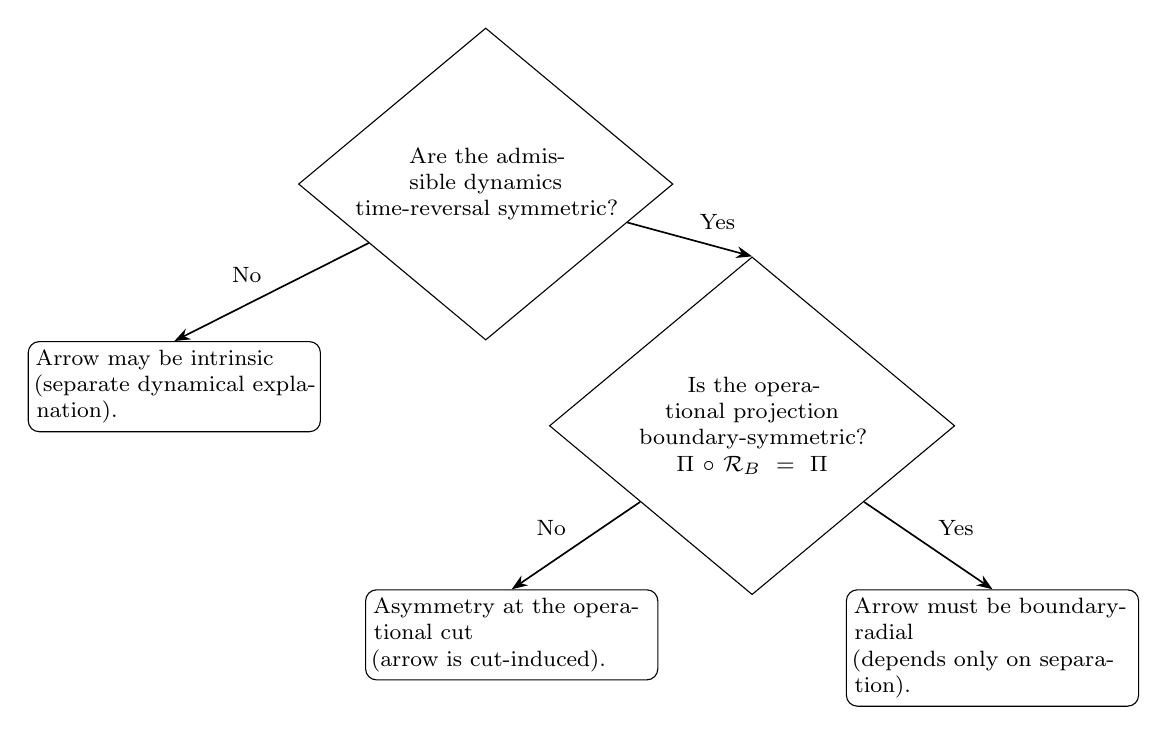
\begin{tikzpicture}[
  font=\footnotesize,
  % 1. Reduced node distance (vertical and horizontal)
  node distance=1.0cm and 0.4cm, 
  >={Stealth[length=2.0mm]},
  decision/.style={
    draw, diamond, aspect=1.2,
    align=center,
    inner sep=1pt,
    % 2. Reduced width to fixed cm or smaller fraction (0.22 vs 0.30)
    text width=3.5cm 
  },
  outcome/.style={
    draw, rounded corners,
    align=left,
    inner sep=3pt,
    % 2. Reduced width to fixed cm or smaller fraction
    text width=3.5cm 
  },
  edge/.style={->, line width=0.6pt} % Slightly thicker for visibility
]

% Root Node
\node[decision] (dynamics)
{Are the admissible dynamics\\time-reversal symmetric?};

% Level 1 Branches
% Use shifting to manually fine-tune if 'below left' is too aggressive
\node[outcome, below left=of dynamics, xshift=-0.5cm] (intrinsic)
{Arrow may be intrinsic\\(separate dynamical explanation).};

\node[decision, below right=of dynamics, xshift=0.5cm] (projection)
{Is the operational projection\\boundary-symmetric?\\$\Pi \circ \mathcal{R}_B = \Pi$};

% Level 2 Branches (Children of Projection)
\node[outcome, below left=of projection, xshift=0.5cm] (cut)
{Asymmetry at the operational cut\\(arrow is cut-induced).};

\node[outcome, below right=of projection, xshift=-0.5cm] (radial)
{Arrow must be boundary-radial\\(depends only on separation).};

% Edges
\draw[edge] (dynamics) -- node[midway, above left] {No} (intrinsic.north);
\draw[edge] (dynamics) -- node[midway, above right] {Yes} (projection.north);

\draw[edge] (projection) -- node[midway, above left] {No} (cut.north);
\draw[edge] (projection) -- node[midway, above right] {Yes} (radial.north);

\end{tikzpicture}
\caption{Diagnostic decision procedure implied by Theorem~\ref{thm:projection-induced-arrows}.
The framework classifies arrow-like directedness by separating intrinsic dynamical asymmetry from projection-induced asymmetry.
When admissible dynamics are symmetric and the operational reduction is boundary-symmetric, any arrow-like diagnostic in the reduced description must be boundary-radial.
Adapted from Theorem~\ref{thm:projection-induced-arrows} and the accompanying remarks on boundary symmetry.}
\label{fig:decision-tree}
\end{figure}

The following worked examples are included solely to operationalize the diagnostic criterion
\(\Pi\circ \mathcal{R}_B=\Pi\) and to illustrate, in concrete terms, the distinction between
projection-induced boundary-radial arrows and cut-introduced asymmetry.
They are not proposed as new mechanisms for any specific arrow, nor as a boundary-selection principle.

\subsection{Worked diagnostic examples}
\label{subsec:worked-diagnostic-examples}

\subsubsection{Example A (Boundary-symmetric projection): coarse-grained macrostate in reversible Hamiltonian dynamics}
\label{sec:exA-thermo}

\paragraph{Setup.}
Consider a classical Hamiltonian system with microstate \(\Gamma\in\Omega\) (phase space),
Hamiltonian flow \(\Phi_t:\Omega\to\Omega\), and time-reversal involution
\(\mathcal{T}:\Omega\to\Omega\) (e.g.\ momentum inversion) satisfying the standard reversibility relation
\begin{equation}
\mathcal{T}\circ \Phi_t = \Phi_{-t}\circ \mathcal{T}.
\label{eq:ham-reversal}
\end{equation}
Let the admissible-history space \(\mathcal{H}\) be the set of trajectories
\(h:\mathbb{R}\to\Omega\) with \(h(t)=\Phi_t(\Gamma_0)\) for admissible initial data \(\Gamma_0\).
Fix a conditioning boundary \(B\) at parameter value \(\lambda_B=0\), and for this example take
\(\lambda=t\) (the theorem does not require this choice, but it is convenient for exposition).

Define the boundary-reflection map on histories by
\begin{equation}
(\mathcal{R}_B h)(t) \;=\; \mathcal{T}\big(h(-t)\big),
\label{eq:RB-ham}
\end{equation}
i.e.\ reflection about \(t=0\) together with microphysical time reversal.

\paragraph{Operational projection.}
Let \(\Pi:\mathcal{H}\to\mathcal{D}\) be the coarse-graining map that sends a microtrajectory
to a macrotrajectory built from a \emph{time-local} macrostate \(M(t)\) defined by a partition
of phase space into macrocells \(\{C_\alpha\}\). Concretely, define
\begin{equation}
M_h(t) \;:=\; \alpha \quad \text{iff}\quad h(t)\in C_\alpha,
\qquad
\Pi(h) \;:=\; \big(M_h(t)\big)_{t\in\mathbb{R}}.
\label{eq:macro-proj}
\end{equation}
Assume the macrocells are defined by time-reversal even constraints
(e.g.\ densities, energies, coarse position bins), so that each macrocell is invariant under \(\mathcal{T}\):
\begin{equation}
\mathcal{T}(C_\alpha)=C_\alpha\quad \text{for all }\alpha.
\label{eq:cell-invariant}
\end{equation}
This is the standard situation for thermodynamic macrostates: the coarse variables discard
microscopic momentum sign structure, phases, and fine correlations.

\paragraph{Verification of boundary symmetry.}
Using \eqref{eq:RB-ham}--\eqref{eq:cell-invariant}, for any history \(h\) and any \(t\),
\[
(\mathcal{R}_B h)(t)=\mathcal{T}(h(-t))\in C_\alpha
\;\;\Longleftrightarrow\;\;
h(-t)\in \mathcal{T}^{-1}(C_\alpha)=C_\alpha.
\]
Thus \(M_{\mathcal{R}_B h}(t)=M_h(-t)\). If the reduced description \(\mathcal{D}\) is taken to encode
macro-quantities as \emph{functions of unsigned separation from the boundary} (as is typical when conditioning
is specified by a preparation at \(t=0\) without recording an absolute orientation tag), then the induced reduced
macrotrajectory is invariant under boundary reflection. One operationally natural way to state this is:
\begin{equation}
\Pi(h)\equiv \Pi(\mathcal{R}_B h)\quad \text{as reduced descriptions anchored at }B,
\label{eq:PiRB-thermo}
\end{equation}
because the coarse macro-information available at separation \(|t|\) from the preparation boundary is identical
for \(h\) and \(\mathcal{R}_B h\) once oriented departure is not part of the recorded reduced state.\footnote{Equivalently:
the experimental macro-protocol reports reduced statistics conditioned only on the preparation event at \(B\),
and does not include an additional variable that labels ``which side'' of the boundary is being traversed.}

This is precisely the boundary-symmetric case of Definition~\ref{def:boundary-symmetric-projection}:
the operational cut does not retain oriented boundary information.

\paragraph{Boundary-radial diagnostics.}
Let \(Q:\mathcal{D}\to\mathbb{R}\) be a direction-sensitive macro-diagnostic (e.g.\ coarse-grained entropy,
distance-to-equilibrium, or a mixing functional). Under \(\Pi\circ\mathcal{R}_B=\Pi\), Lemma~1 applies, so
\begin{equation}
\mathbb{E}[Q\circ \Pi]\;=\;F\!\left(\operatorname{sep}(t,0)\right)=F(|t|),
\label{eq:Qr-thermo}
\end{equation}
i.e.\ the diagnostic can vary only with separation from the conditioning boundary. In particular, the special
case of monotone \(F\) corresponds to familiar one-sided ``relaxation'' narratives once an orientation convention
is imposed externally, but the theorem itself requires only the boundary-radial dependence.

\paragraph{Operational test.}
This case admits a direct operational check: prepare the same macro-boundary condition at \(B\) and compare
reduced statistics at equal separations on either side of the boundary under a protocol that does not record
an orientation label. Boundary symmetry corresponds to indistinguishability of the reduced statistics for
boundary-reflected preparations at equal \(\operatorname{sep}(t,0)=|t|\). Failure of such indistinguishability constitutes empirical evidence that the projection is boundary-asymmetric in the sense of Definition~\ref{def:boundary-symmetric-projection}.

\subsubsection{Example B (Boundary-asymmetric projection): retaining an oriented boundary label in the reduced description}
\label{sec:exB-asym}

\paragraph{Purpose.}
This example shows how boundary symmetry can fail \emph{even when admissible dynamics remain symmetric},
and how such failure is classified by the framework as asymmetry introduced at the level of the operational cut.
The construction is intentionally simple: the reduced description retains an explicit oriented boundary label.

\paragraph{Setup.}
Let the admissible dynamics and boundary reflection \(\mathcal{R}_B\) be as in Example~A (or any other symmetric
admissible-history space). Fix the same conditioning boundary \(B\) at \(\lambda_B=0\).

\paragraph{Boundary-asymmetric projection.}
Define a reduced description \(\mathcal{D}'\) that contains both the coarse macrostate \(M_h(t)\) and an explicit
\emph{side-of-boundary tag} \(\sigma(t)\in\{+1,-1\}\) indicating the orientation relative to \(B\):
\begin{equation}
\sigma(t):=\operatorname{sgn}(t)
\quad (\sigma(0):=0\ \text{by convention}),\qquad
\Pi'(h)\;:=\;\big(M_h(t),\sigma(t)\big)_{t\in\mathbb{R}}.
\label{eq:Pi-prime}
\end{equation}
Then, for \(t\neq 0\),
\[
\Pi'(h)\neq \Pi'(\mathcal{R}_B h),
\]
because \(\sigma(t)\) flips sign under boundary reflection: \(\sigma(t)\mapsto \sigma(-t)=-\sigma(t)\).
Thus
\begin{equation}
\Pi'\circ \mathcal{R}_B \neq \Pi',
\label{eq:PiRB-fails}
\end{equation}
so boundary symmetry fails \emph{by construction at the level of the reduced description}.

\paragraph{Classification.}
This is not a counterexample to Theorem~\ref{thm:projection-induced-arrows}. It is an instance of the failure mode already described in
Remark~1: the operational cut preserves oriented boundary information, so the boundary-symmetric theorem
does not apply. In such cases, any observed directedness can be attributed (in whole or in part) to the
\emph{asymmetric content of the projection itself} rather than to the admissible dynamics.

\paragraph{Are such projections ``standard''?}
In many standard physical reduced descriptions, orientation relative to a conditioning boundary is \emph{not}
encoded as an additional state variable; the reduced description is specified by preparation at \(B\) together
with statistics as a function of separation from that preparation.
However, orientation-labeled reductions like \eqref{eq:Pi-prime} can occur in practice whenever an operational
protocol explicitly records ``before/after'' or ``pre/post'' labels, or when an external clock variable is carried
into the reduced record as a signed offset from the conditioning event.
The framework therefore treats such cases as neither pathological nor disallowed: they are simply outside the
boundary-symmetric class and are classified accordingly.

\paragraph{Operational diagnostic.}
The same operational criterion applies: if two boundary-reflected preparations yield different reduced statistics
because the reduced record retains an orientation tag, then \(\Pi\circ\mathcal{R}_B=\Pi\) fails and the arrow-like
directedness is cut-introduced.

The following domain-specific illustrations can be read as implicit applications of this diagnostic procedure.

\paragraph{Takeaway.}
Examples~\ref{sec:exA-thermo} and \ref{sec:exB-asym} together make the diagnostic procedure explicit:
under symmetric admissible dynamics, boundary-radial arrows follow when the operational projection is
boundary-symmetric, and need not follow when the projection preserves oriented boundary information.

\subsection{Thermodynamic coarse-graining}

Classical statistical mechanics provides canonical instances in which reversible
microscopic dynamics coexist with macroscopic entropy increase. Hamiltonian
phase-space flow preserves volume and admits time-reversed trajectories, yet
coarse-grained descriptions exhibit relaxation toward equilibrium
\cite{Boltzmann1896,Jaynes1957}.

Within the present framework, the arrow does not attach to the microdynamics but
to the operational projection defining macrostates. Conditioning boundaries are
introduced implicitly through preparation procedures, macrostate definitions,
or coarse-graining anchors. Entropy increase then measures separation from such
boundaries under the reduced description, rather than intrinsic temporal flow of
the admissible dynamics.

\subsection{Quantum measurement and decoherence}

In quantum theory, unitary dynamics preserve reversibility at the level of the
global state, while reduced descriptions obtained by tracing out environmental
degrees of freedom display decoherence, relaxation, and apparent irreversibility.
Preparation, factorization, and measurement events naturally serve as conditioning
boundaries for such reduced descriptions
\cite{Zurek2003,Schlosshauer2007}.

From the present perspective, decoherence-induced arrows are boundary-radial:
coherence measures decay as separation from the conditioning boundary increases.
No intrinsic arrow is attributed to the underlying unitary evolution; directedness
appears only after projection discards system--environment correlations beyond
operational resolution.

\subsection{Computational and information-theoretic arrows}

Reversible computation offers a particularly transparent illustration of the
distinction between admissible dynamics and operational arrows. Classical
reversible logic gates (e.g.\ Toffoli or Fredkin gates) and unitary quantum circuits
implement bijective transformations at the admissible level, admitting
time-reversal symmetry in the relevant sense.

Operational arrows arise only when projections are introduced, most notably
through measurement, reset, or erasure. Logical erasure is a paradigmatic
projection: many distinct logical states are mapped to a single standard state,
discarding logical degrees of freedom. Initialization, reset, or measurement
events thereby function as conditioning boundaries.

In this setting, apparent computational directedness---progress from input to
output, information loss, or entropy production in physical implementations---is
boundary-relative. It attaches to the operational cuts required to obtain usable
computational states, not to the reversible core dynamics themselves. Landauer-type
results connect such projections to thermodynamic costs, but the structural origin
of the arrow lies in the projection and its boundary, not in the admissible logic
or unitary evolution \cite{Landauer1961}.

\subsection{General diagnostic role of boundaries}

Across these examples, the role of the conditioning boundary is uniform. Changing
the boundary---for example, by post-selection, reset, or alternative preparation
protocols---changes the apparent arrow without modifying the underlying admissible
structure. This highlights the diagnostic utility of the framework: whenever
arrow-like behavior is observed in a reduced description governed by symmetric
admissible dynamics, the source of directedness must be traced to the operational
projection and its anchoring boundary.
\section{Relation to Prior Work}

The emergence of arrow-like directedness from time-reversal symmetric descriptions
has a long history in statistical mechanics, quantum foundations, and
information theory. The present work is aligned with these traditions in spirit,
but differs in emphasis by stating an explicit structural constraint. Under
minimal symmetry and reduction assumptions, direction-sensitive diagnostics in reduced descriptions must be boundary-radial,
i.e.\ functions only of separation from an operational conditioning boundary.

Early treatments by Boltzmann established that thermodynamic irreversibility does
not arise from microscopic laws themselves, but from coarse-grained descriptions
of phase space \cite{Boltzmann1896}. Subsequent developments emphasized the role
of typicality and macrostates, while leaving open the question of why a particular
temporal orientation is selected.

Information-theoretic approaches, particularly those associated with Jaynes,
recast statistical mechanics as inference under constraints, locating entropy
increase in the updating of incomplete descriptions rather than in fundamental
dynamics \cite{Jaynes1957}. The present framework is compatible with this view,
and formalizes the role of conditioning boundaries implicit in such updates.

In quantum theory, environment-induced decoherence and measurement models explain
the appearance of irreversibility through the tracing out of environmental degrees
of freedom \cite{Zurek2003}. Here, preparation, factorization, and measurement
events naturally function as conditioning boundaries, while the underlying unitary
dynamics remain symmetric. Related perspectival and relational approaches emphasize
that physical states and properties are defined relative to systems or observers
\cite{Rovelli1996}.

Recent philosophical analyses have clarified the distinction between fundamental
time symmetry and emergent arrows, often invoking cosmological boundary conditions
such as the Past Hypothesis \cite{Price1996}. The present result does
not compete with such proposals, but instead constrains the form that any arrow
explanation must take once operational reduction is acknowledged, independently
of how a particular boundary is selected.

Finally, Landauer’s principle highlights the connection between logical
irreversibility and physical entropy production, identifying erasure as a
many-to-one mapping at the informational level \cite{Landauer1961}. In the present
framework, logical erasure is a paradigmatic projection, and its associated arrow is boundary-relative to the erasure/reset operation rather than intrinsic to the reversible computational core.

Overall, this work may be viewed as complementary to existing thermodynamic,
quantum, and information-\allowbreak theoretic accounts: it does not propose a new mechanism
for irreversibility, but articulates a general constraint on how arrow-like
directedness can arise in reduced descriptions of symmetric admissible dynamics.
\section{Discussion, Limits, and Extensions}

\subsection{Diagnostic Consequences of the Projection Constraint}
\label{subsec:diagnostic-consequences}

Theorem~\ref{thm:projection-induced-arrows} functions not as a generative model but as a
\emph{structural no-go constraint} on admissible explanations of arrow-like directedness.
This subsection makes explicit several immediate diagnostic consequences.
These are not additional assumptions or empirical claims, but logical corollaries
that follow directly from the formal core and classify arrow-like diagnostics by the locus of asymmetry, excluding entire classes of arrow explanations.

\begin{corollary}[Arrow-Origin Classification]
Any arrow-like diagnostic defined on a reduced description must originate from
exactly one of the following sources:
\begin{enumerate}
\item asymmetry in the admissible dynamics themselves,
\item asymmetry in the operational projection,
\item asymmetry introduced by boundary selection.
\end{enumerate}
No arrow-like directedness can arise intrinsically from symmetric admissible dynamics
under boundary-symmetric projection.
\end{corollary}

\begin{remark}
This corollary provides a classification scheme rather than a mechanism.
It partitions arrow explanations by the locus at which asymmetry enters,
independent of the physical domain under consideration.
\end{remark}

\begin{remark}[Forced disclosure]
The structural strictness of the theorem may appear tautological: if direction is excluded
from the projection, it cannot appear in the diagnostic.
This apparent tautology is precisely the diagnostic content of the result.
It compels any account of arrow-like behavior to explicitly identify the specific locus of
asymmetry it relies upon-whether in the admissible dynamics, the operational cut,
or the selection of a conditioning boundary-rather than allowing such asymmetry
to remain implicit or disguised as an emergent feature of symmetric laws.
\end{remark}

\begin{corollary}[Structural Impossibility of Intrinsic Arrows]
In the absence of asymmetry in admissible dynamics, projection, or boundary selection,
direction-sensitive diagnostics on the reduced description are structurally impossible.
\end{corollary}

\begin{remark}
This is a no-go constraint in the standard sense:
a single counterexample---i.e.\ a reduced diagnostic that violates boundary-radial
dependence while satisfying the assumptions of the theorem---would falsify the result.
The corollary does not assert that intrinsic arrows never occur, only that their
existence requires explicit asymmetry.
\end{remark}

\begin{corollary}[Boundary-Reflection Test]
\label{cor:boundary-reflection-test}
If a proposed arrow diagnostic is invariant under boundary reflection at the level of
the reduced description, then it is necessarily projection-induced and boundary-radial.
Conversely, any diagnostic that depends on the sign of separation from the boundary
must violate at least one of the theorem’s assumptions.
\end{corollary}

\begin{remark}
This corollary provides an operational test:
it determines whether an observed arrow reflects intrinsic directional structure
or is an inevitable artifact of projection and conditioning.
The theorem therefore constrains \emph{form}, not magnitude or dynamics.
\end{remark}

\begin{remark}[On Falsifiability]
Like other structural constraints (e.g.\ no-cloning or Bell-type inequalities),
the present theorem is falsifiable without being numerically predictive.
It restricts what forms arrow-like explanations may take, rather than predicting
specific values or time evolutions.
\end{remark}

\noindent
Corollary~\ref{cor:boundary-reflection-test} is operationalized explicitly in
Examples~\ref{sec:exA-thermo} and~\ref{sec:exB-asym}, where boundary-reflected preparations
yield indistinguishable reduced statistics under boundary-symmetric projection (Example~A),
and distinguishable statistics when oriented boundary information is retained in the reduced description (Example~B).
See Sec.~\ref{subsec:worked-diagnostic-examples} for the concrete operational construction.

Concrete operational realizations of this test are summarized in Box 1.

\paragraph{Falsifiability.}
Although the present result is a structural constraint rather than a predictive model, it is falsifiable in the standard sense applicable to no-go theorems. The theorem would be falsified by the exhibition of all three of the following conditions simultaneously:
\begin{enumerate}
\item \emph{Symmetric admissible dynamics:} an admissible-history space $\mathcal{H}$ equipped with a boundary reflection $\mathcal{R}_B$ such that $\mathcal{R}_B(h)\in\mathcal{H}$ for all $h\in\mathcal{H}$ and $\mathcal{R}_B^2=\mathrm{id}$;
\item \emph{Boundary-symmetric operational reduction:} an operational projection $\Pi:\mathcal{H}\to\mathcal{D}$ satisfying $\Pi\circ\mathcal{R}_B=\Pi$;
\item \emph{Oriented reduced diagnostics:} a diagnostic quantity $Q:\mathcal{D}\to\mathbb{R}$ whose expectation value depends on the \emph{sign} of departure from the conditioning boundary, i.e.\ on $\operatorname{sgn}(\lambda(h)-\lambda_B)$,
+where $\operatorname{sgn}$ denotes the sign of the oriented departure,
where $\operatorname{sgn}$ denotes the sign of the oriented departure rather than solely on the unsigned separation $\operatorname{sep}(\lambda(h),\lambda_B)$.
\end{enumerate}
The existence of such a case would demonstrate intrinsically oriented arrow-like behavior emerging from symmetric admissible dynamics under boundary-symmetric operational reduction, thereby directly contradicting Theorem~\ref{thm:projection-induced-arrows}. To our knowledge, no such counterexample has been identified in thermodynamic, quantum, or computational settings.

\paragraph{Interpretive remark.}
This falsifiability criterion clarifies the empirical content of the framework: the theorem does not preclude the existence of arrows, but restricts the circumstances under which they may arise. Any observed direction-sensitive diagnostic must therefore be traceable to a verifiable failure of at least one of the stated assumptions-through intrinsic dynamical asymmetry, boundary-asymmetric projection, or explicit boundary-selection principles.

\subsection{Diagnostic Application: Boltzmann’s H-Theorem}
\label{sec:diagnostic-h-theorem}

Textbook treatments of the Boltzmann H-theorem commonly present entropy increase as a
consequence of purely mechanical dynamics. In a standard formulation, the Boltzmann
equation-together with Liouville’s theorem-is taken to imply monotonic decrease of the
functional $H=\int f\ln f\,d\Gamma$, thereby demonstrating irreversible approach to
equilibrium despite underlying time-reversal symmetric microdynamics
(e.g.\ \citep[Sec.~1.4]{Pathria2011}).

At face value, this presentation suggests that arrow-like directedness emerges from
symmetric admissible dynamics through statistical reasoning alone. The present framework
allows this claim to be examined diagnostically by identifying the locus at which
directional asymmetry enters.

\paragraph{Admissible dynamics and projection.}
At the microscopic level, the admissible dynamics are Hamiltonian and time-reversal
symmetric: for every admissible trajectory in phase space, the momentum-reversed
trajectory is also admissible. The reduced description is provided by the single-particle
distribution function $f(\mathbf{r},\mathbf{p},t)$, obtained by projecting the full
$N$-particle distribution onto one-particle marginals. This projection discards
higher-order correlations and is fixed relative to the reduced description.

\paragraph{Implicit boundary asymmetry.}
A crucial ingredient in the derivation of the Boltzmann equation is the molecular chaos
assumption (Stosszahlansatz), which asserts that particle velocities are uncorrelated
\emph{prior} to collision. This assumption is imposed at a chosen reference time and
propagated forward under the kinetic equation. Importantly, no corresponding assumption is
made about the absence of correlations after collision.

From the standpoint of admissible histories, this asymmetry does not arise from the
Hamiltonian dynamics themselves, nor from the coarse-graining projection as such. Rather,
it reflects a privileged treatment of correlations relative to a conditioning boundary:
correlations are constrained on one side of the boundary (before collision or at an
initial reference time) but not on the other.

\paragraph{Boundary-reflection diagnostic.}
Applying the operational test articulated in Sec.~\ref{subsec:diagnostic-consequences}, one
may ask whether boundary-reflected preparations-obtained by reversing momenta and
correlations at the conditioning boundary-yield indistinguishable reduced statistics under
the same projection. In the presence of the molecular chaos assumption, they do not: the
Boltzmann equation itself fails to be invariant under such reflection because the
assumption singles out a direction of correlation propagation.

Accordingly, the condition $\Pi\circ\mathcal{R}_B=\Pi$ does not hold for the kinetic
description used in the H-theorem derivation. The arrow-like behavior diagnosed by the
monotonic decrease of $H$ therefore does not arise from boundary-symmetric projection acting
on symmetric admissible dynamics.

\paragraph{Classification.}
Within the present taxonomy, the H-theorem exemplifies a case of \emph{boundary-selection
asymmetry}. The entropy increase it describes is boundary-radial relative to a specific
conditioning choice-low correlations at the reference boundary-but this boundary is not
fixed or selected by the mechanical dynamics alone. Claims that the H-theorem derives
irreversibility purely from symmetric mechanics must therefore be understood as incomplete:
a boundary-selection principle is structurally required.

\paragraph{Corrected statement.}
A formulation consistent with the present framework is the following: given symmetric
Hamiltonian dynamics and a boundary condition imposing low correlations at a reference
boundary, entropy increases away from that boundary under the Boltzmann equation. The arrow
thus reflects the imposed boundary asymmetry rather than an intrinsic directionality of the
admissible dynamics.

\begin{center}
\fbox{
\begin{minipage}{0.95\linewidth}
\textbf{Box 1: Operational Tests for Boundary-Symmetric Projection}

\vspace{0.5em}

The boundary-symmetry condition $\Pi \circ \mathcal{R}_B = \Pi$ is not a matter of
representation, but of operational indistinguishability. The following table
summarizes concrete experimental protocols for assessing boundary symmetry across
domains.

\vspace{0.5em}

\newcolumntype{Y}{>{\raggedright\arraybackslash}X}
\newcolumntype{P}[1]{>{\raggedright\arraybackslash}p{#1}}
\begin{tabularx}{\linewidth}{|P{2.9cm}|P{2.9cm}|Y|Y|}
\hline
\textbf{Domain} &
\textbf{Conditioning Boundary $B$} &
\textbf{Forward Protocol} &
\textbf{Boundary-Reflected Protocol} \\
\hline

Classical Statistical Mechanics &
Preparation at $t=0$ &
Prepare macrostate $M$, evolve to $t=+\tau$, measure macro-variables &
Prepare $M$ with momentum-reversed microstates, evolve to $t=-\tau$, measure macro-variables \\
\hline

Quantum Decoherence &
System--environment factorization &
Prepare $\rho_S\otimes\rho_E$, evolve unitarily, trace over environment &
Prepare time-reversed joint state, evolve under reversed Hamiltonian, trace over environment \\
\hline

Reversible Computation &
Memory initialization &
Initialize register, execute circuit, record output &
Reverse circuit without output recording (output readout itself defines a boundary) \\
\hline
\end{tabularx}

\vspace{0.5em}

If the reduced statistics obtained from the forward and boundary-reflected protocols
are indistinguishable, the operational projection is boundary-symmetric.
Failure of indistinguishability constitutes empirical evidence that oriented boundary
information is retained by the projection.
\end{minipage}
}
\end{center}

\subsection{Boundary Selection as a Structural Constraint}

The present framework does not propose a mechanism for the selection of a
conditioning boundary. This is a deliberate restriction rather than a gap, and
reflects the paper’s aim to isolate structural necessity from contingent physical
or cosmological inputs. The contribution of the theorem is to isolate boundary
selection as a distinct explanatory axis: any account of arrow-like directedness
must either (i) posit intrinsic asymmetry in the admissible dynamics, or (ii)
supply a boundary-selection principle explaining why a particular conditioning
boundary is physically realized. Hybrid accounts that appeal to
projection-induced irreversibility while implicitly privileging a boundary are
thereby rendered conceptually explicit.

In this sense, the framework does not relocate the arrow problem arbitrarily, but
forces a sharp separation between the \emph{origin of directedness} (projection
relative to a boundary) and the \emph{origin of boundary selection}. Clarifying
this separation is itself a form of explanatory progress: it prevents asymmetric
assumptions from being silently imported into accounts that otherwise appeal only
to symmetric dynamics and operational reduction, and it prevents conflation of
structural necessity with contingent physical, cosmological, or pragmatic
conditions.

Related discussions of boundary selection and its explanatory role appear, for example,
in analyses of the Past Hypothesis and in broader treatments of temporal arrows
\cite{Wallace2010,Carroll2010}; the present result is orthogonal to such accounts,
constraining admissible forms of arrow explanations without proposing a selection principle.

Boundary-selection principles-cosmological, dynamical, pragmatic, or observer-
relative-may therefore be introduced as orthogonal inputs without altering the
structural result established here. Such principles determine which boundary is
realized; they do not, by themselves, explain why reduced descriptions exhibit
arrow-like diagnostics once conditioning is imposed.

\subsection{Limits of applicability}

The results of this paper rely on two core assumptions: symmetric admissible
dynamics and information-losing operational reduction. If primary admissible
dynamics violate time-reversal symmetry, the theorem does not apply as stated.
In that regime, the framework nevertheless retains diagnostic value by sharply
separating intrinsic asymmetry in the dynamics from projection-induced
asymmetry in reduced descriptions.

Known violations of time-reversal symmetry in the weak interaction (e.g.\ neutral meson systems)
are classified within this framework as \emph{intrinsic dynamical asymmetries}.
Their existence constitutes a failure of the symmetry assumption for that specific sector,
but does not alter the present constraint on arrows arising in effective sectors
(thermodynamic, computational) where admissible dynamics are symmetric.

Similarly, if an operational description preserves directional information by
construction-by encoding asymmetry directly into the operational projection
itself-then boundary-radial behavior need not follow. Such cases fall outside the
scope of the present analysis, which is restricted to projections that treat
admissible histories symmetrically relative to the conditioning boundary.

By contrast, objective collapse models (e.g.\ GRW, Penrose) fall outside the boundary-symmetric
class considered here by positing intrinsically time-asymmetric, non-unitary admissible dynamics.
They are thereby classified as introducing arrows at the dynamical level (Type~1),
distinct from the projection-induced arrows (Type~2) that characterize standard quantum
measurement and decoherence accounts.

\subsection{Extensions and future directions}

Potential extensions of the framework follow naturally from its diagnostic
character: once arrow-like quantities are understood as measures of separation
from a conditioning boundary, information-theoretic and geometric generalizations
become especially natural. Such extensions include explicit
formulations of diagnostic quantities in information-theoretic terms (e.g.\ mutual information relative to a conditioning boundary), as well as applications to 
gravitational or causal horizons treated as operational boundaries. These directions may be pursued without relaxing the minimal assumptions that underwrite the present constraint theorem.

We note that if the global spacetime manifold itself lacks a reflection symmetry
due to topological constraints-e.g.\ differing initial and final singularity structures-
this constitutes an intrinsic asymmetry of the admissible histories, placing it
outside the boundary-symmetric class constrained here.
\section{Conclusion}

We presented a minimal, trajectory-first constraint framework in which arrow-like directedness arises
as an inevitable feature of operational descriptions anchored at conditioning boundaries.
Under time-reversal symmetric admissible dynamics and fixed information-losing projections,
direction-sensitive diagnostics are constrained to be boundary-radial. Unique intrinsic
arrows require additional explicitly asymmetric assumptions.

This reframes arrow puzzles as questions about operational cuts and boundary selection,
rather than about fundamental temporal directedness in the underlying admissible structure itself.
% ============================================================
% Appendix A: Explicit Toy Derivation (Boundary-Radiality)
% Purpose: make Lemma 1 visibly derivational, not definitional.
% ============================================================

\appendix
\section{Explicit Toy Derivation of Boundary-Radiality}
\label{app:toy-derivation}

This appendix provides a minimal derivation illustrating how boundary-radial dependence follows
from (i) symmetric admissible dynamics and (ii) an information-losing operational projection
anchored at a conditioning boundary. No physical assumptions are used; the construction is
purely structural. The point is not to model any particular arrow, but to make explicit why
direction-sensitive diagnostics on a reduced description cannot survive boundary-reflection
identification.

\subsection{Setup: admissible histories, boundary reflection, projection}

Let $\mathcal{H}$ be a finite set of admissible histories. No preferred ordering or parameter is assumed
at this level; $\mathcal{H}$ is simply the admissible-history space.

Fix a conditioning boundary $B$ and assume the admissible structure admits an involutive
\emph{boundary reflection} (pairing) map
\begin{equation}
\mathcal{R}_B : \mathcal{H} \to \mathcal{H}, \qquad \mathcal{R}_B^2 = \mathrm{id}.
\end{equation}
Intuitively, $R_B$ pairs each admissible history with the history obtained by reflecting
its admissible realization with respect to the boundary condition $B$ (as defined in
Sec.~\ref{sec:formal-core}). The only property required here is involution.

Let $\Pi$ be an operational projection to a reduced description space $\mathcal{D}$,
\begin{equation}
\Pi : \mathcal{H} \to \mathcal{D} \equiv \Pi(\mathcal{H}),
\end{equation}
assumed to be \emph{boundary-symmetric} in the sense of Sec.~\ref{sec:formal-core}:
\begin{equation}
\Pi \circ \mathcal{R}_B = \Pi .
\label{eq:toy-boundary-sym}
\end{equation}
Equation~\eqref{eq:toy-boundary-sym} is the formal expression of the idea that the reduced
description identifies boundary-reflected admissible histories: operationally, histories
related by $\mathcal{R}_B$ are indistinguishable after projection.

Finally, let $Q$ be any diagnostic defined purely on the reduced description:
\begin{equation}
Q : \mathcal{D} \to \mathbb{R}.
\end{equation}
The diagnostic may be interpreted as ``arrow-like'' only insofar as it is direction-sensitive
at the reduced level; this appendix shows that such sensitivity cannot depend on the sign of
separation from the boundary.

\subsection{Minimal example: explicit pairing and identification}

Consider the smallest nontrivial case where boundary reflection produces nontrivial pairings:
\begin{equation}
\mathcal{H} = \{h_1, h_2, h_3, h_4\}.
\end{equation}
Define an involution $R_B$ by pairing histories into two reflected pairs:
\begin{equation}
\mathcal{R}_B(h_1)=h_2,\quad \mathcal{R}_B(h_2)=h_1,\qquad
\mathcal{R}_B(h_3)=h_4,\quad \mathcal{R}_B(h_4)=h_3.
\label{eq:toy-involution}
\end{equation}
Let the projection $\Pi$ identify each reflected pair:
\begin{equation}
\Pi(h_1)=\Pi(h_2)=d_A,\qquad
\Pi(h_3)=\Pi(h_4)=d_B,
\label{eq:toy-projection}
\end{equation}
so that $\mathcal{D}=\{d_A,d_B\}$ and $\Pi \circ \mathcal{R}_B = \Pi$ holds identically.

\subsection{Derivation: invariance of reduced diagnostics under boundary reflection}

Using only the boundary-symmetry condition~\eqref{eq:toy-boundary-sym}, for any $h\in \mathcal{H}$ we have
\begin{equation}
\Pi(h) = \Pi(\mathcal{R}_B h).
\end{equation}
Applying any reduced diagnostic $Q$ yields
\begin{equation}
Q(\Pi(h)) = Q(\Pi(\mathcal{R}_B h)).
\label{eq:toy-diagnostic-invariance}
\end{equation}
In the explicit example~\eqref{eq:toy-involution}--\eqref{eq:toy-projection},
Eq.~\eqref{eq:toy-diagnostic-invariance} reads
\begin{equation}
Q(d_A)=Q(\Pi(h_1))=Q(\Pi(h_2)), \qquad
Q(d_B)=Q(\Pi(h_3))=Q(\Pi(h_4)),
\end{equation}
i.e.\ the diagnostic cannot distinguish members within a boundary-reflected pair.

\subsection{From invariance to boundary-radiality}

To connect the above invariance to the boundary-radial form used in Lemma~1, introduce any
parameter structure $(\mathcal{S}, \mathrm{sep}, \lambda_B)$ in the sense of
Sec.~\ref{sec:formal-core}, where $\lambda$ is a parametrization along histories and
$\mathrm{sep}(\lambda,\lambda_B)\ge 0$ is the induced unsigned separation from the boundary
value $\lambda_B$. Boundary reflection acts by sign reversal around $\lambda_B$:
\begin{equation}
R_B : \lambda \mapsto \lambda' \ \ \text{with}\ \ \lambda' - \lambda_B = -(\lambda - \lambda_B),
\end{equation}
so that
\begin{equation}
\mathrm{sep}(\lambda,\lambda_B)=\mathrm{sep}(\lambda',\lambda_B).
\label{eq:toy-sep-invariant}
\end{equation}
Boundary-symmetry of $\Pi$ implies that any reduced observable or diagnostic is constant on
$\mathcal{R}_B$-orbits, i.e.\ depends only on the equivalence class $[h]=\{h, \mathcal{R}_B h\}$.
By Eq.~\eqref{eq:toy-sep-invariant}, the most general dependence compatible with this
identification is therefore a function of the \emph{unsigned} separation:
\begin{equation}
Q(\Pi(h)) = f\!\left(\mathrm{sep}(\lambda(h),\lambda_B)\right)
\end{equation}
for some function $f$ (possibly piecewise, depending on the coarse equivalence classes induced
by $\Pi$). In particular, no diagnostic definable on $D$ can depend on the \emph{sign} of
$\lambda-\lambda_B$ without violating $\Pi\circ \mathcal{R}_B=\Pi$.

\subsection{Interpretive remark (structural, not mechanistic)}

The conclusion is purely structural: whenever an information-losing projection identifies
boundary-reflected admissible histories, direction-sensitive diagnostics on the reduced
description cannot encode an intrinsic ``which-way'' dependence. Any arrow-like directedness
visible after projection must be boundary-radial, i.e.\ indexed only by separation from the
conditioning boundary. This is the toy instantiation of Lemma~1 in Sec.~\ref{sec:formal-core}.

\bibliographystyle{unsrt}
\bibliography{bib/references}

\end{document}